This chapter describes the general workflow we propose within this work. This workflow can be seen in Figure~\ref{img-workflow}. To start off, some kind of software product line is required. It's source code has to be structured in a way that allows for an algorithm to recognize the individual features as well as their interrelations, as these can be very costly to implement by hand.

{\color{red} Pfeil von Fragebogen zu Generator sollte zu der Selektion zeigen.}

\begin{figure}[H]
	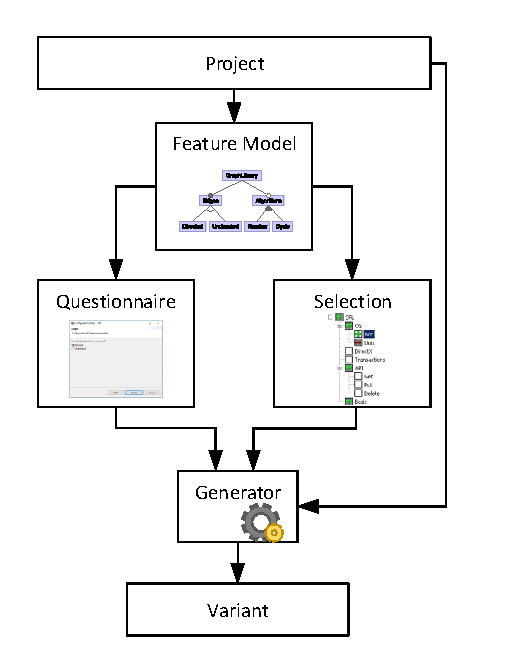
\includegraphics{img/img-workflow.pdf}
	\caption{Diagram showing the general workflow}
	\label{img-workflow}
\end{figure}

The two major steps of extraction of the feature model and the creation and usage of the questionnaire are described in detail in the following sections. As a final result of these steps stands a product targeting the users needs.


\subsection{Extraction of a Feature Model}
Out of the given structure of the source code base we extract the hierarchies of the features as well as additional dependencies. These are the input for the automated generation of a feature model. This allows for overview over the product line and it's variability. During our efforts to implement an automated generation of a feature model we encounter some problems for which we have to find solutions or workarounds.

The first challenge consists of finding the structures of the given source code and processing them programmatically. Most software complies to conventions regarding the naming and structuring of directories. We try to make use of these conventions. However, in most source code there are violations within their own conventions. Instead of interrupting the whole process, we implement error handling. The result is a notification for the user to alert the developers about the error. Also, the remaining information, which aren't immediately affected by the error, are still extracted and used for the generation of the feature model, if possible.

Another challenge lies within the order of processing the features during the creation of the feature model. To correctly reproduce the hierarchy of the features, features have to be declared as child features of their parents. If the declared parent feature doesn't already exist, the creation of a feature model fails. So we have to ensure for each feature, that it gets processed after it's parent feature.

Another error we found is one or more features having a parent feature which doesn't exist as a code artifact itself. Thus, the parent feature doesn't exists in the feature model and it's child features can't be placed in the hierarchy in the correct place. To still include these features in the feature model we create an {\color{red}abstract feature (Zitat)} for the parent feature. The abstract feature is a direct child of the root feature. As it doesn't have any describing code, it only has a name and no additional descriptive details.

In each step of the creation of the feature model, e.g. after adding a feature or constraint to the feature model, it is checked by a SAT-solver to avoid creating an invalid feature model (represented by a void object) which has no valid configurations (see section~\ref{ch:sat}). The extracted feature model is also used in the following step of configuration. There, it visualizes the interrelations of the features and supports the understanding of the configuration steps.


\subsection{Questionnaire Approach}
Configuration is a challenging tasks within the scope of software product lines. The resulting feature model from the automated generation yields a better overview over the possible features and their interrelationships. Although the formalism of a feature model allows for tool support for the process of configuration, still domain knowledge is required to be able to find the right combination of features for a given use-case.

This work introduces a method allowing experts to apply their knowledge and understanding to a whole product line during the development. Whenever a variation is configured using the questionnaire, the user benefits from the invested domain knowledge.

In this work, we made the decision to use a questionnaire-based approach \cite{qbvm}. In the progress of implementation, experts also design a questionnaire. They do so in such a way, that a user has to answer a given amount of questions to perform the configuration of a product. Depending on the implementation of the questionnaire, a partial or even complete configuration can be archived by a user through just answering the questions of the questionnaire.

The selection of features gets lifted to a higher level of abstraction. The user only has to decide between the possible answers presented to him in the questionnaire to best fit to his use-case. Internally the selected answers are mapped to a specified (de-)selection of features. This way the user avoids the hassle of considering implementation-details of each feature. This effectively redesigns the process of configuration in such a way, that a user is independent of the knowledge about the details of the implementation and can focus on tailoring the product line to his specific use-case.

\subsection{Questionnaire Implementation}

The quality of the resulting variation highly depends on the implementation of the questionnaire during development. Our work therefore introduces a set of tools to easily integrate such a questionnaire. The following paragraphs will give an overview over the possible definitions of a questionnaire.

{\color{red} TODO: add screenshots}

Each page of the questionnaire is defined independently. It always contains at least a question and more than one possible answer. The answers can be grouped analogous to the grouping of features in a feature model: \textit{or} (at least one answer has to be selected), \textit{alternative} (exactly one answer has to be selected) and \textit{and} (any number of answers can be selected).

Each answer internally has a mapping to a set of features. In the case a specific answer is chosen, the corresponding features are selected or deselected as specified.

Each answer can also have an indicator to define which page of the questionnaire should be displayed next. An answer can also indicate the end of the questionnaire. If no next page is defined the questionnaire will continue with the next page within it's definition. This allows a dynamic conditional design of the questionnaire so the user is only confronted with the exact set of questions needed to configure the variant for his specific use-case. This also allows the user to skip questions or cancel the configuration before finishing it and thus creating a partial configuration.

We also introduce a data structure to hold the definition of a questionnaire. To archive easy integration we decided for a definition in XML. We defined the necessary tags to create a questionnaire which are displayed in Figure~\ref{fig:xmlFigure}.

\begin{figure}[H]
\begin{tabulary}{\linewidth}{LLL}
\textbf{Tag} & \textbf{attributes} & \textbf{child tags}\\
\hline
configurationSurvey & & projectName, section, page\\
section & id & name, description\\
page & id, sectionId & question, answers\\
answers & type & answer\\
answer & nextPageId & label, description, dependencies\\
dependencies & & feature\\
feature & selection & \\
\end{tabulary}\vspace{2.5em}
\end{figure}

The individual tags are explained as follows:
\begin{itemize}
\item \texttt{configurationSurvey}: The root tag to contain all other tags for the questionnaire.
\item \texttt{section}: Enables grouping of question-pages. Also displays the name and description at the top of every page.
\item \texttt{page}: Contains a question and the corresponding answers. Also has an indicator for a section
\item \texttt{answers}: Contains the individual possible answers and groups them in the specified manner.
\item \texttt{answer}: Defines the displayed text of an answer as well as the corresponding features. Can also have an indicator for the next page.
\item \texttt{dependencies}: Defines the (un-)selection of features, if the corresponding answer gets selected.
\end{itemize}

\begin{figure}[H]
	\lstset{language=XML}
	\begin{lstlisting}
	<configurationSurvey>
		<projectName>Name</projectName>
		<section id="0">
			<name>Section Name</name>
			<description>Section description</description>
		</section>
		<page id="0" sectionId="0">
			<question>Question for the user</question>
			<answers type="alternative">
				<answer nextPageId="1">
					<label>Answer label</label>
					<description>
						Answer description
					</description>
					<dependencies>
						<feature selection="false">
							Unselected feature
						</feature>
						<feature>selected feature</feature>
					</dependencies>
				</answer>
			</answers>
		</page>
	</configurationSurvey>
	\end{lstlisting}
	\caption{Examplary XML file for a  questionnaire}
	\label{fig:xmlFigure}
\end{figure}

This allows for experts to design a questionnaire in such a way, that it can guide a user without specific domain knowledge throughout the whole process of configuration. Through just answering questions concerning his specific use-case the user takes all necessary decisions. After he completes the questionnaire, our tool maps his answers to a complete configuration, which is then applied to the existing code artifacts. Finally, a working product is the result.